%%%%%%%%%%%%%%%%%%%%%%%%%%%%%%%%%%%%%%%%%%%%%%%%%%%%%%%%%%%%%%%%%%%%%%%%%%%%%%
\section{Degrader geometry}

The pion degrader was introduced to suppress the background to \piplusenu\
from muon decays in flight and was thought of as a disk made of non-magnetic material
inserted into the beam for the calibration runs and moved out of the beam
during the data taking.

Making the degrader of CH2 allows to use the process of radiative capture of
stopped $\pi^-$'s on hydrogen, $\pi^-p \to n\gamma$, for calibrating the Mu2e momentum scale
at full field. RPC on H2 yields 129.4 MeV photons. For that, a converter ring of a larger radius needs to be added.

For now, implement a converter ring $R_{out}$ = 250mm, with $R_{in}$ defined
by the converter thickness.

\piplusenu\ studies: the degrader disk thickness of 4 mm Ti is close to optimal.

4mm of Ti is equivalent to about $1.8 g/cm^2$.
\begin{itemize}
\item
  9mm CH2 + 1.0mm Pb: : 2.0 $g/cm^2$   .. $\pi*15^2*(0.9*0.95 + 0.08*11.34): \simeq 2 g/cm^2$
\item
   9mm CH2 + 0.8mm Pb: : $1.76 g/cm^2$
 \item
   reduce the outer radius of the degrader disk - don't need 15 cm
 \item
   CH2 disk R=14 cm, weight        : $0.9*0.95*\pi*14^2$ = 526 gr \\
   Pb  foil R=10cm thickness 0.8mm : 0.08*11.34*314    = 285 gr \\
   total                           : 811 gr
\end{itemize}

To make sure that $e^+$ and $e^-$ do not cross the converter foil multiple times,
move the converter forward by 1cm.

In the real degrader, the converter foil will be supported
by a carbon foam disk, to be designed.

%%%%%%%%%%%%%%%%%%%%%%%%%%%%%%%%%%%%%%%%%%%%%%%%%%%%%%%%%%%%%%%%%%%%%%%%%%%%%%
\subsection{Converter thickness - connection to \piplusenu\  calibration}

\begin{figure}[H]
  \begin{tikzpicture}
    \node[anchor=south west,inner sep=0] at (0,0.) {
      % \node[shift={(0 cm,0.cm)},inner sep=0,rotate={90}] at (0,0) {}
      \makebox[\textwidth][c] {
        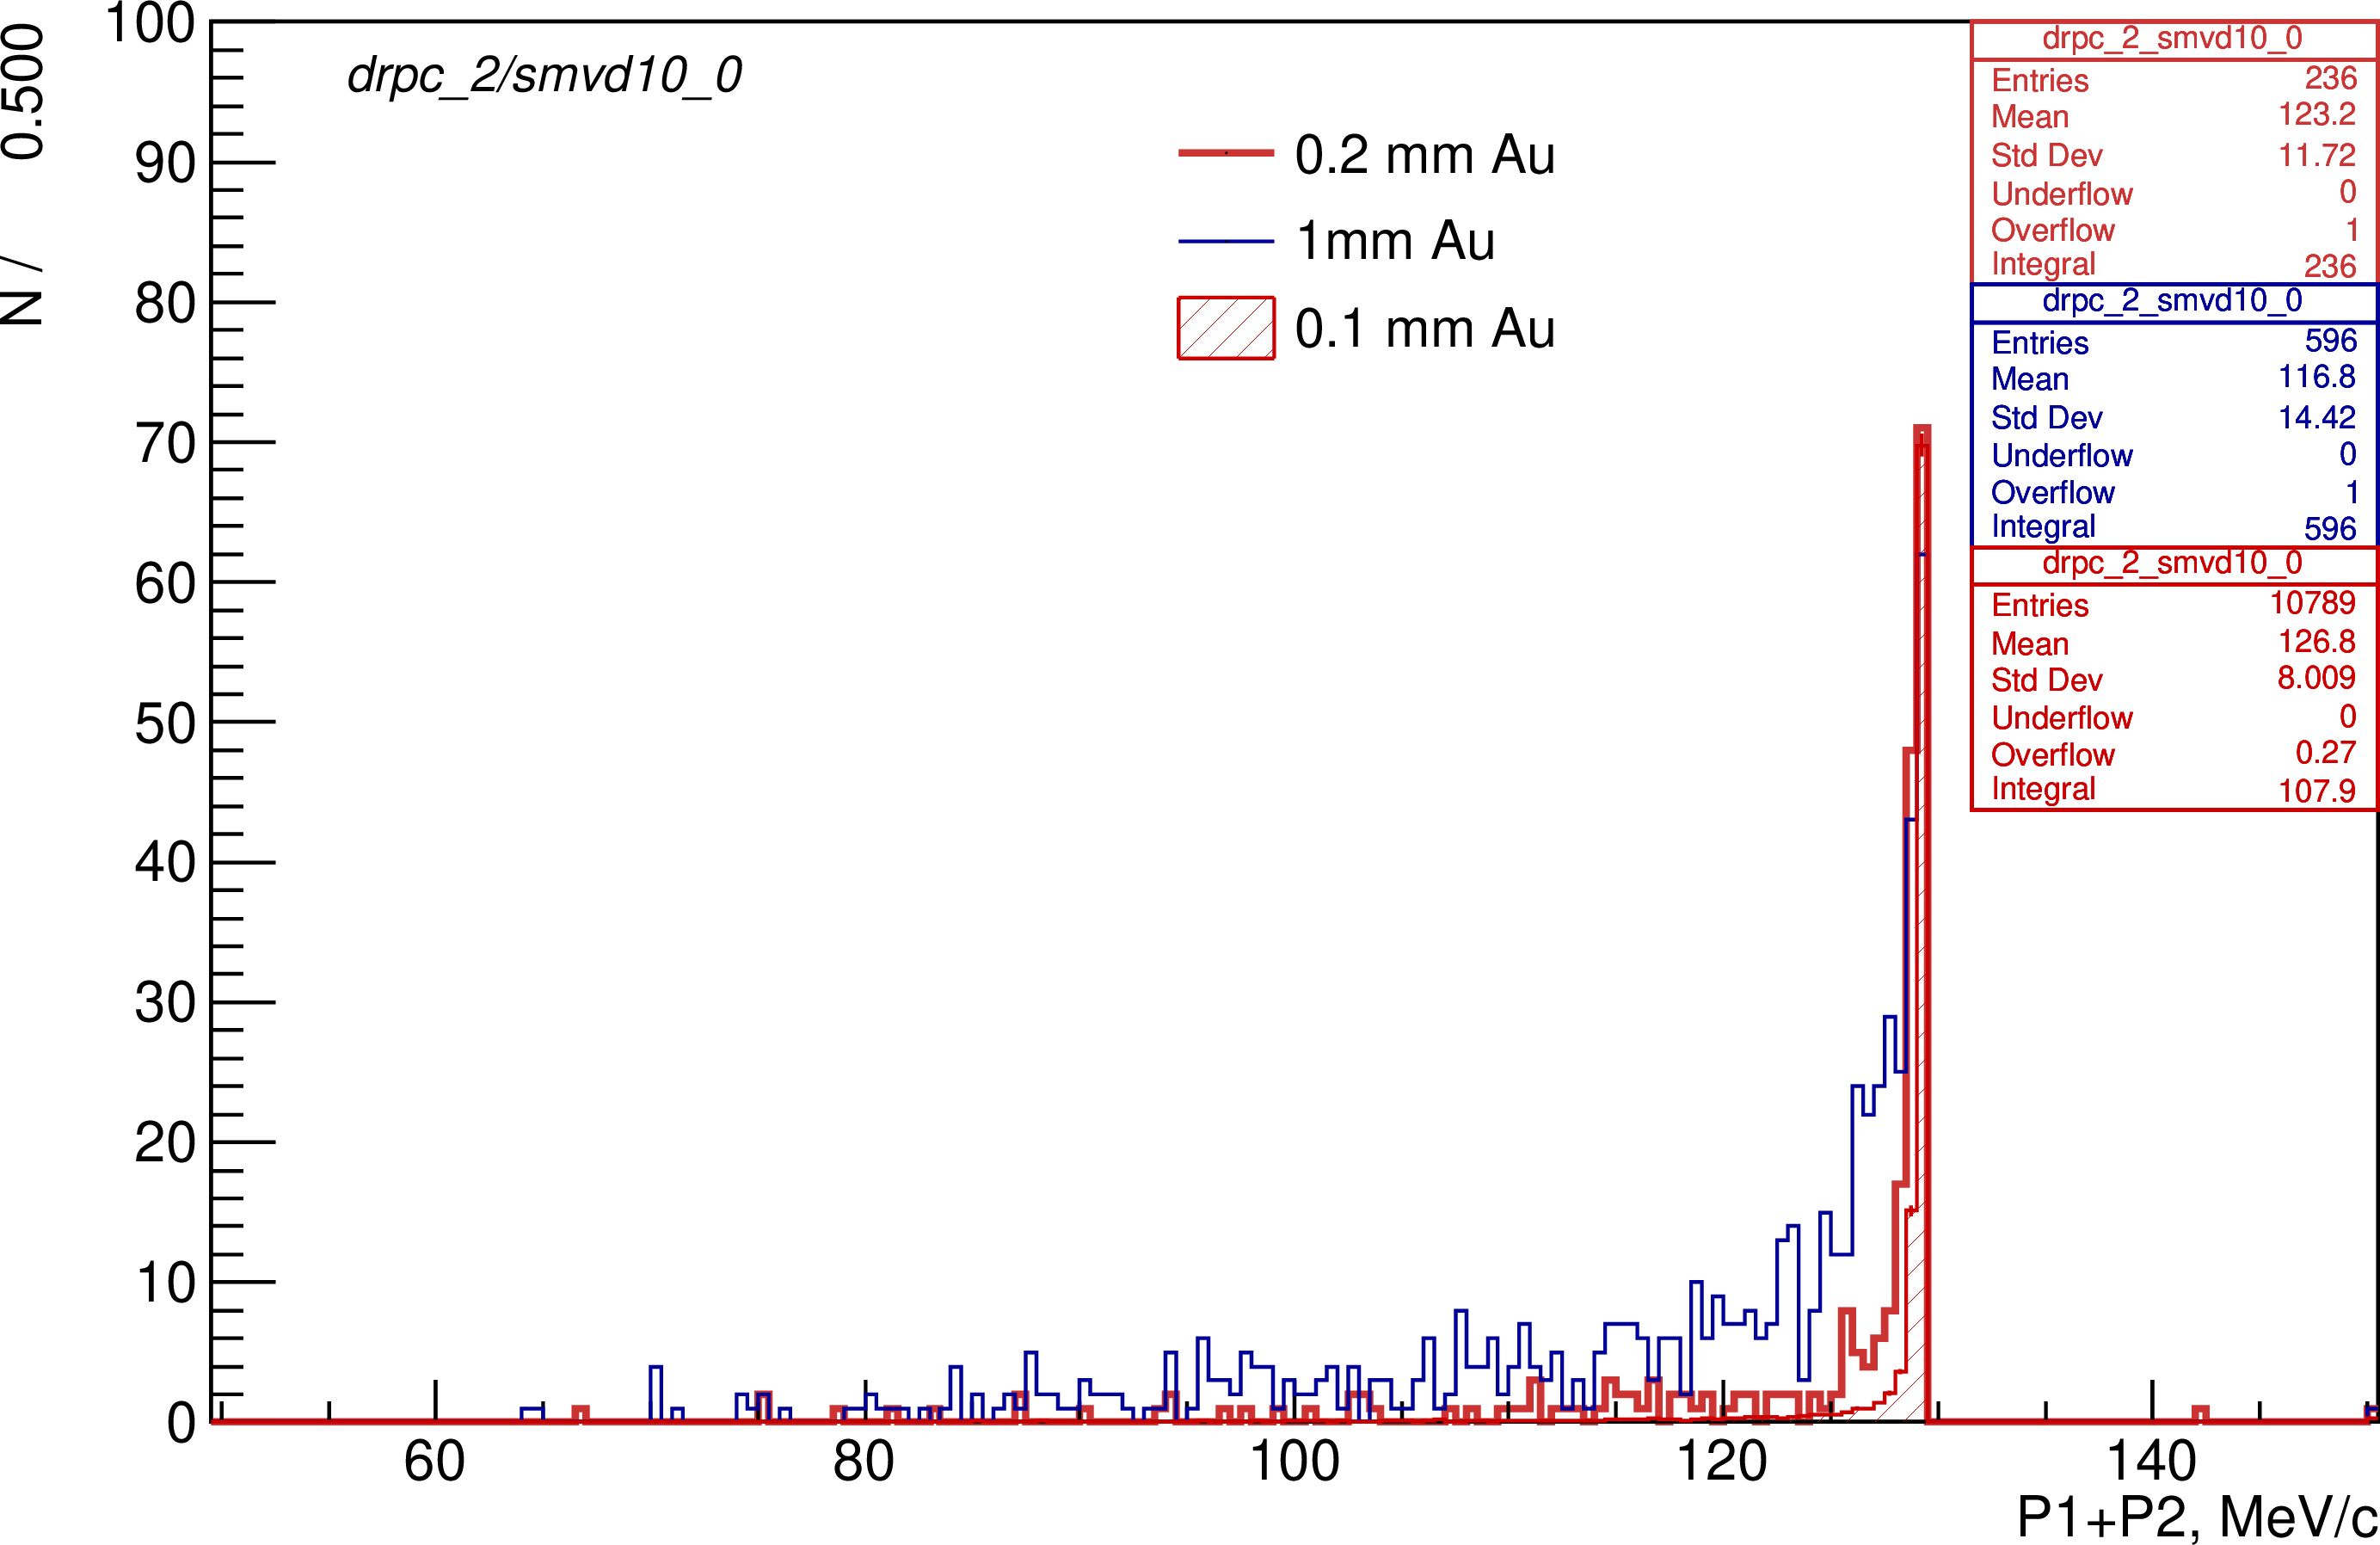
\includegraphics[width=0.9\textwidth]{pdf/figure_00010}
      }
    };
    % \node [text width=8cm, scale=1.0] at (14.5,0.5) {$\mu_B$, expected background mean};
    % \node [text width=8cm, scale=1.0, rotate={90}] at (1.5,7.5) { $S_{D}$, ``discovery'' signal strength  };
  \end{tikzpicture}
  \caption{
    \label{figure:sum_mom_vd10}
    P1+P2 at VD10
  }
\end{figure}

\begin{figure}[H]
  \begin{tikzpicture}
    \node[anchor=south west,inner sep=0] at (0,0.) {
      % \node[shift={(0 cm,0.cm)},inner sep=0,rotate={90}] at (0,0) {}
      \makebox[\textwidth][c] {
        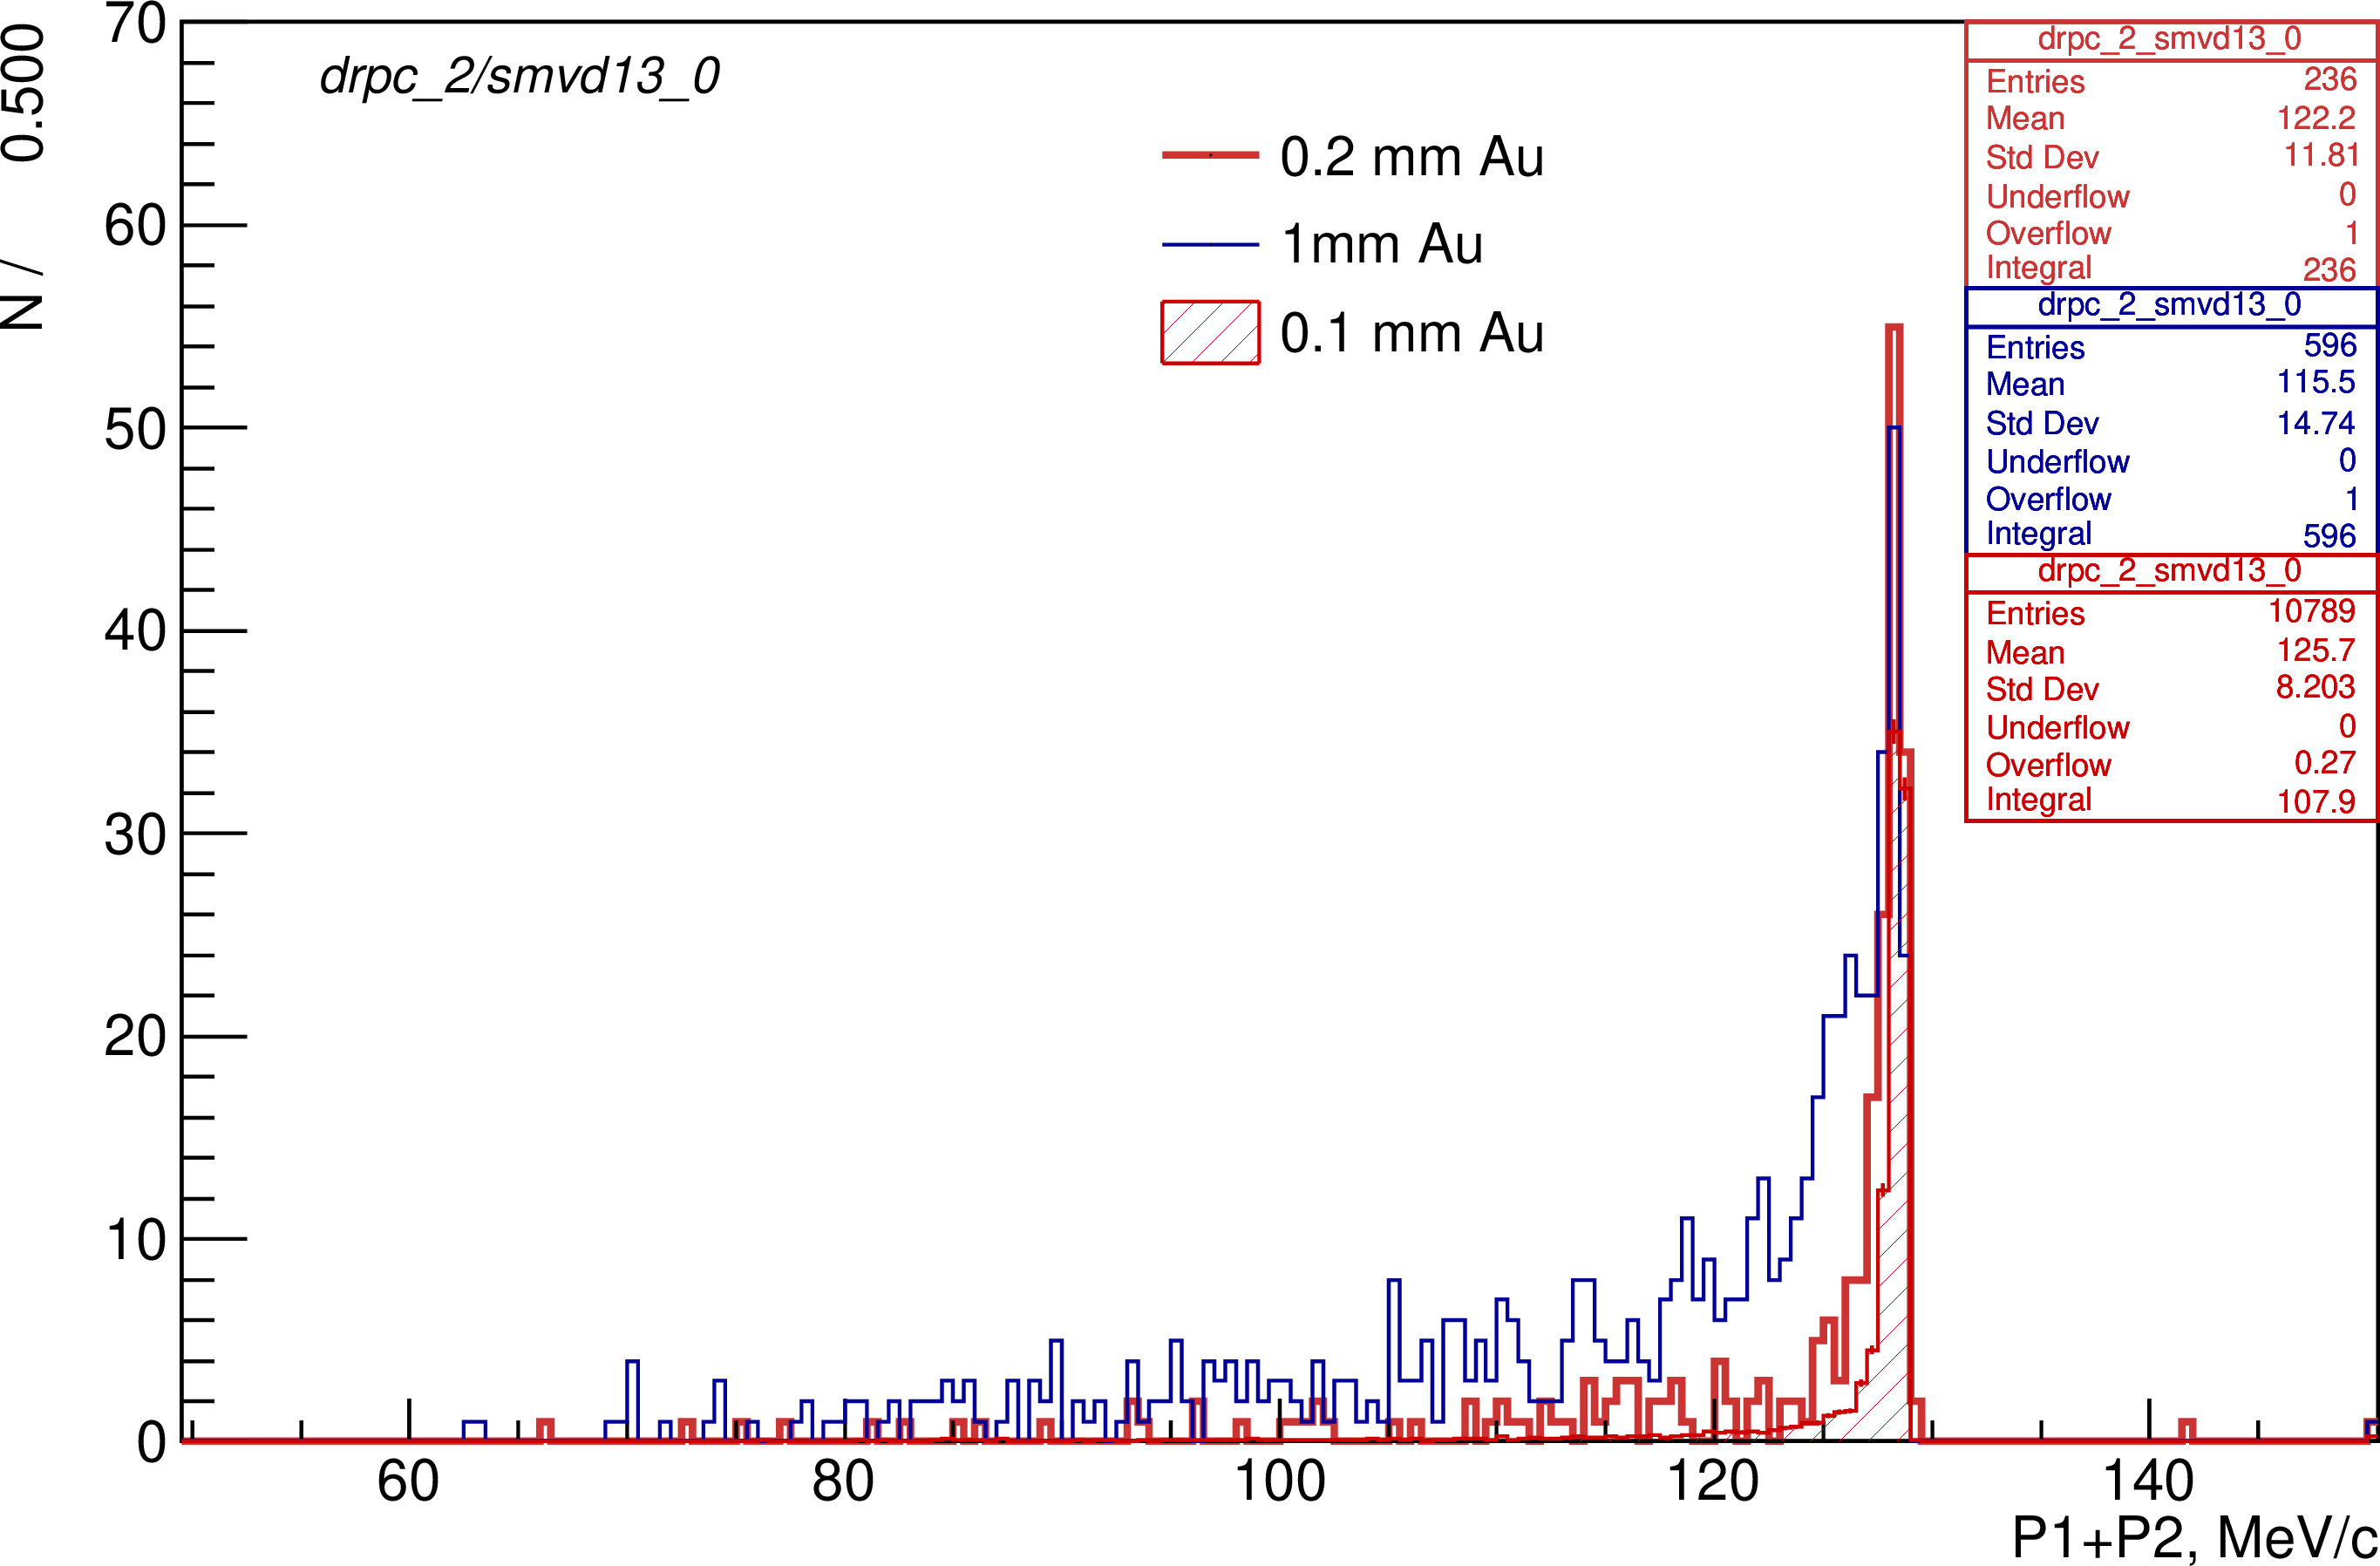
\includegraphics[width=0.9\textwidth]{pdf/figure_00013}
      }
    };
    % \node [text width=8cm, scale=1.0] at (14.5,0.5) {$\mu_B$, expected background mean};
    % \node [text width=8cm, scale=1.0, rotate={90}] at (1.5,7.5) { $S_{D}$, ``discovery'' signal strength  };
  \end{tikzpicture}
  \caption{
    \label{figure:sum_mom_vd13}
    P1+P2 at VD13
  }
\end{figure}

The converter thickness is chosen based on the distributions shown in Figure~\ref{figure:sum_mom_vd13}.
Plotted: $P_{tot} = P_1 + P_2$ at VD13, virtual detector in front of the tracker fro events with
two particles, an electron and a positron with P > 30 MeV/c and producing 20 or more straw hits in the tracker each.
Such particles provide a good proxy to the reconstructable tracks.

The event yield increases with the converter thickness. However of interest for the scale calibration only
are the events close to the kinematic edge.
The highest yield of events with P > 128 Mev/c corresponds to the 100 um gold foil, and that determines
the choice of 100 um thick converter.

%%% Local Variables:
%%% mode: latex
%%% TeX-master: t
%%% End:
